\chapter{Results and discussion}
\label{results}
\section{Data collection}
\label{results:collection}

\section{Face and landmark detection}
\label{results:fd}

\begin{figure}
    \centering
    \begin{subfigure}[b]{0.3\textwidth}
      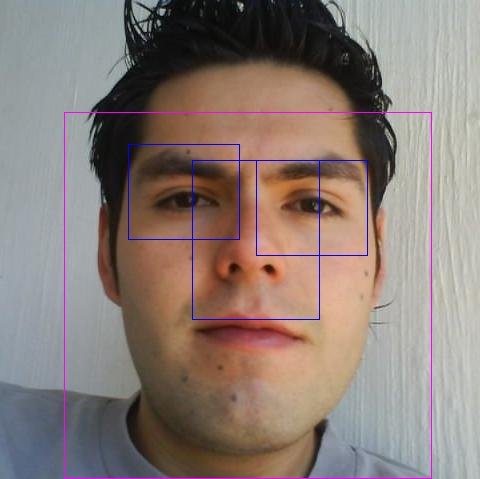
\includegraphics[width=\textwidth]{figures/results/detected_cff0618f-f631-4b0d-80d9-f582fee46fad}
      \caption{Score=1.4313}
      \label{fig:results:fd:good_detected1}
    \end{subfigure}
    \begin{subfigure}[b]{0.3\textwidth}
      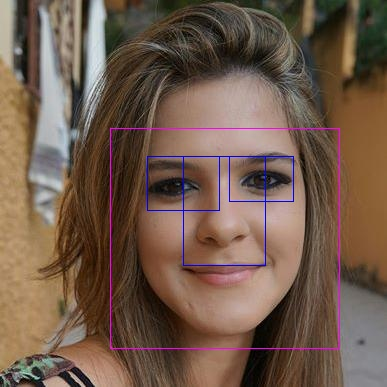
\includegraphics[width=\textwidth]{figures/results/detected_50508cb1-814e-4374-bf07-cef5c301c3c0}
      \caption{Score=1.20387}
      \label{fig:results:fd:good_detected2}
    \end{subfigure}
    \begin{subfigure}[b]{0.3\textwidth}
      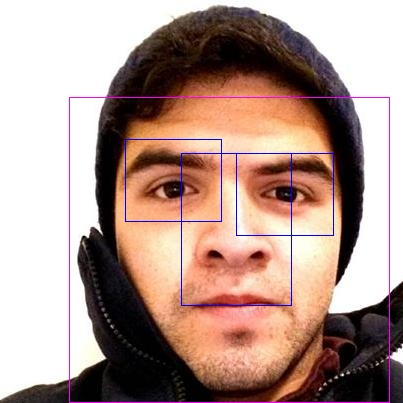
\includegraphics[width=\textwidth]{figures/results/detected_da153846-1afe-4b36-880a-bf8764bfd935}
      \caption{Score=1.09232}
      \label{fig:results:fd:good_detected3}
    \end{subfigure}
\caption{Three examples of high-scoring face detections.}
\label{fig:results:fd:good_detected}
\end{figure}

\begin{figure}
    \centering
    \begin{subfigure}[t]{0.3\textwidth}
      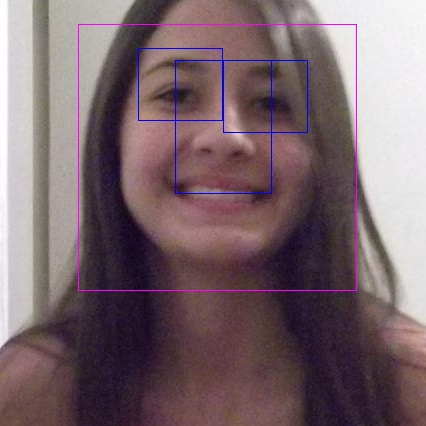
\includegraphics[width=\textwidth]{figures/results/detected_q3_15c3f02d-31c6-4955-8d05-c05029cdb473}
      \caption{Face detection with score=0.0651244 in upper quartile}
      \label{fig:results:fd:q3_detected2}
    \end{subfigure}
    \begin{subfigure}[t]{0.3\textwidth}
      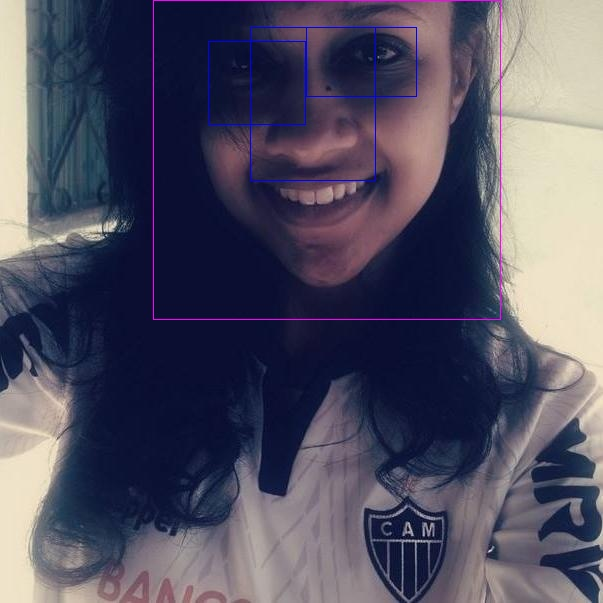
\includegraphics[width=\textwidth]{figures/results/detected_median_fcb1d3ed-7867-40ba-9691-8cd1f59dc36b}
      \caption{Face detection with score=-0.108765 around the median}
      \label{fig:results:fd:median_detected1}
    \end{subfigure}
    \begin{subfigure}[t]{0.3\textwidth}
      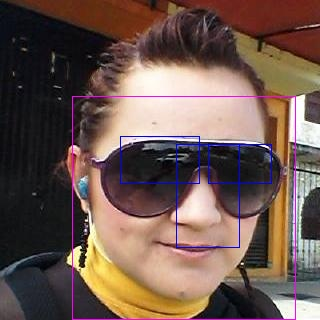
\includegraphics[width=\textwidth]{figures/results/detected_q1_f1c5f486-1697-4089-9bb6-7962d7db630c}
      \caption{Face detection with score=-0.517613 in lower quartile}
      \label{fig:results:fd:q1_detected3}
    \end{subfigure}
\caption{Examples of inferior face pictures. Cropped foreheads, blurriness, sunglasses and small faces are some obvious reasons why a face detection might have received a low score.}
\label{fig:results:fd:other_detected}
\end{figure}

\begin{figure}
    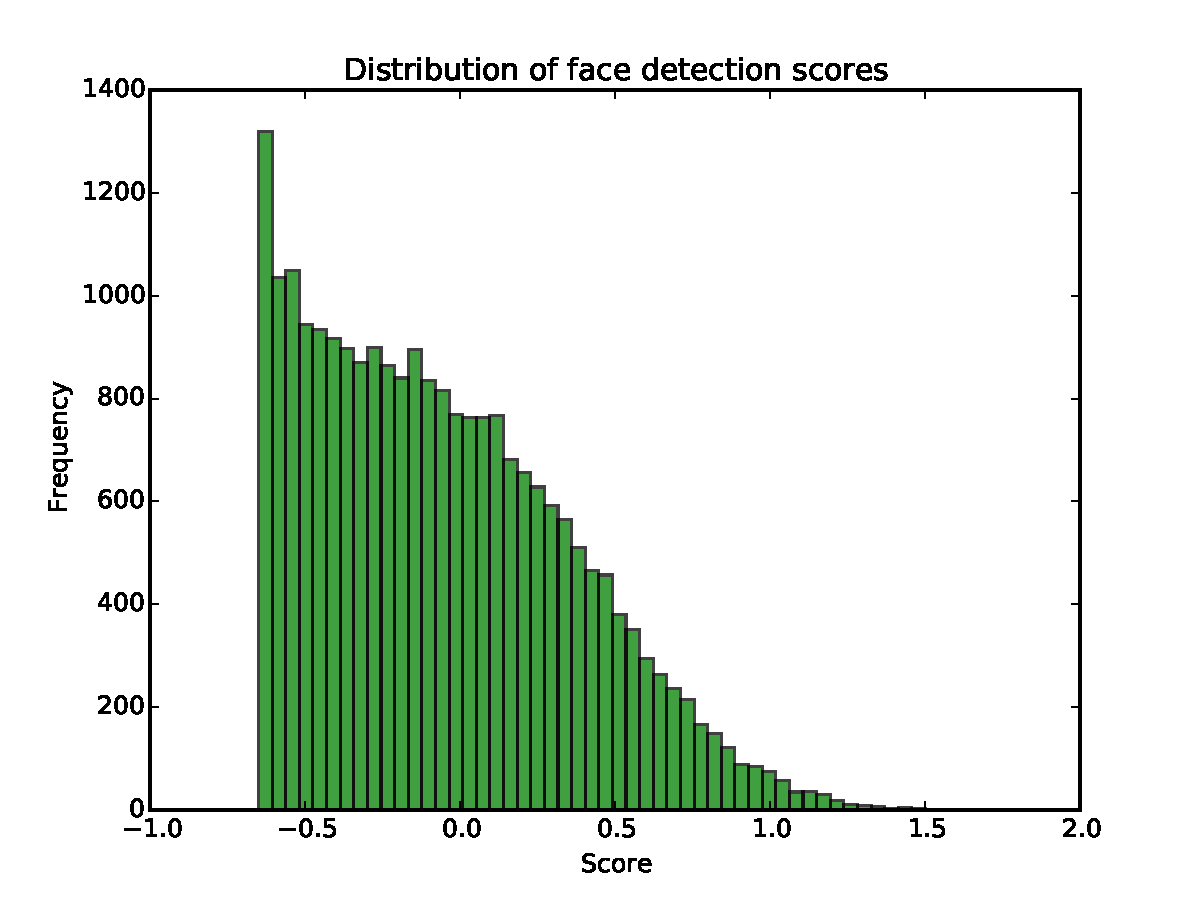
\includegraphics[width=\textwidth]{figures/results/scores_hist}
    \caption{Histogram of scores given by the face detection algorithm to 23379 pictures.}
    \label{fig:results:fd:scores_hist}
\end{figure}


%%% Local Variables: 
%%% mode: latex
%%% TeX-master: "thesis"
%%% End: 
